\chapter{Resultados} \label{chap:resultados}

\subsubsection{Cinemática Directa}
\begin{figure}[H] 
	\centering
	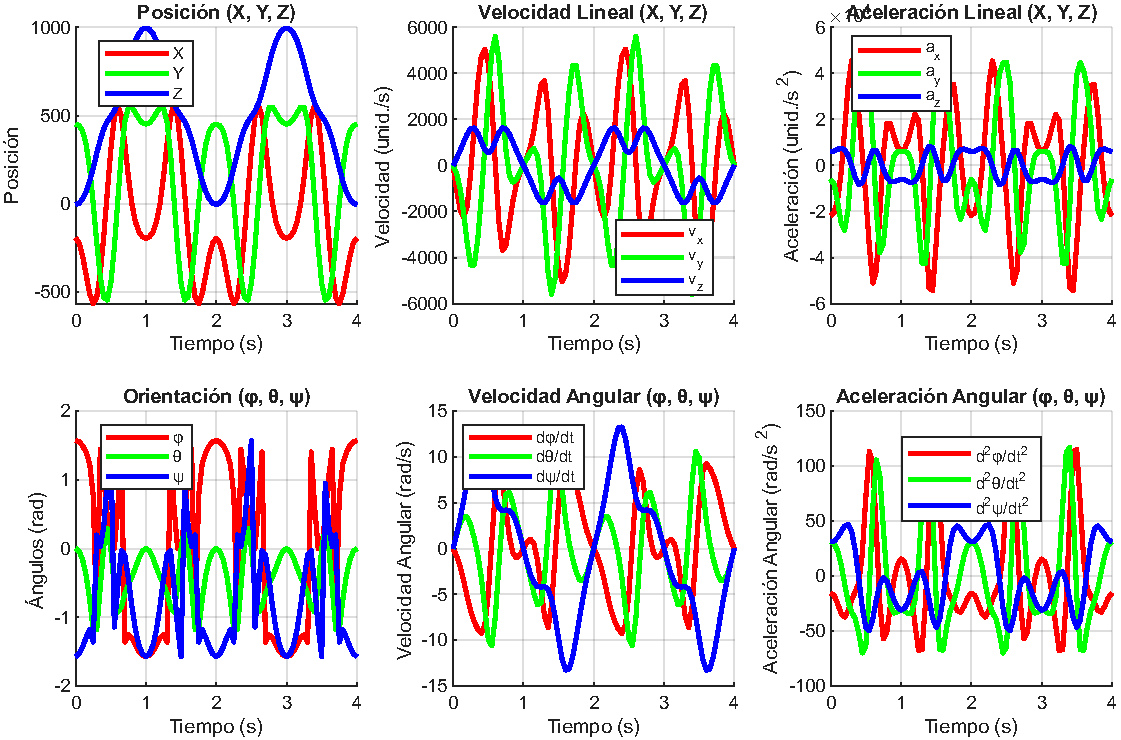
\includegraphics[width=0.8\textwidth]{Graficas_directa_robot_final.pdf}
	\caption{Gráficas cinemática directa en MATLAB.}
	\label{fig:TablasCinematicaDirecta}
\end{figure}

 
 El siguiente conjunto de gráficas representa el comportamiento cinemático de un robot, obtenido mediante la \textbf{cinemática directa} empleando los \textbf{parámetros de Denavit-Hartenberg (DH)}. Cada gráfico describe la evolución de diferentes variables en función del tiempo durante una trayectoria simulada.
 
 \begin{enumerate}
 	\item \textbf{Posición (X, Y, Z)} \\
 	\textit{Gráfica superior izquierda}
 	
 	Muestra la trayectoria espacial del extremo del robot en coordenadas cartesianas.
 	
 	El eje $X$ (rojo), $Y$ (verde) y $Z$ (azul) indican cómo varía la posición en cada uno de los tres ejes con el tiempo.
 	
 	\textbf{Interpretación}: el robot sigue una trayectoria oscilatoria en los tres ejes, lo que sugiere un movimiento complejo, posiblemente cíclico o programado con funciones senoidales o polinomiales.
 	
 	\item \textbf{Velocidad Lineal ($V_x$, $V_y$, $V_z$)} \\
 	\textit{Gráfica superior central}
 	
 	Representa la primera derivada temporal de la posición, es decir, cómo cambia la posición respecto al tiempo.
 	
 	Muestra la rapidez con la que el extremo del robot se mueve en cada dirección.
 	
 	\textbf{Interpretación}: se observa un comportamiento oscilatorio, indicando aceleraciones y desaceleraciones constantes. Las diferencias de amplitud entre ejes indican que el movimiento no es uniforme en todas las direcciones.
 	
 	\item \textbf{Aceleración Lineal ($a_x$, $a_y$, $a_z$)} \\
 	\textit{Gráfica superior derecha}
 	
 	Corresponde a la segunda derivada temporal de la posición.
 	
 	Informa sobre los cambios en la velocidad: aceleraciones positivas y negativas.
 	
 	\textbf{Interpretación}: los valores muestran picos bruscos y cambios rápidos, lo que sugiere que el robot experimenta variaciones rápidas en su movimiento, comunes en trayectorias con alta frecuencia de cambio o maniobras precisas.
 	
 	\item \textbf{Orientación ($\phi$, $\theta$, $\psi$)} \\
 	\textit{Gráfica inferior izquierda}
 	
 	Refleja la orientación del extremo del robot, típicamente representada en ángulos de Euler: roll ($\phi$ - rojo), pitch ($\theta$ - verde) y yaw ($\psi$ - azul).
 	
 	\textbf{Interpretación}: las oscilaciones indican que el robot cambia continuamente su orientación mientras sigue la trayectoria. La transición entre ángulos también sugiere rotaciones complejas, lo cual es habitual en brazos robóticos que deben mantener orientación específica.
 	
 	\item \textbf{Velocidad Angular ($\frac{d\phi}{dt}$, $\frac{d\theta}{dt}$, $\frac{d\psi}{dt}$)} \\
 	\textit{Gráfica inferior central}
 	
 	Representa la velocidad a la que cambian los ángulos de orientación.
 	
 	\textbf{Interpretación}: se identifican zonas de alta velocidad angular, lo que puede indicar maniobras de reorientación rápidas del efector final. El comportamiento es no uniforme y dependiente del ángulo específico.
 	
 	\item \textbf{Aceleración Angular ($\frac{d^2\phi}{dt^2}$, $\frac{d^2\theta}{dt^2}$, $\frac{d^2\psi}{dt^2}$)} \\
 	\textit{Gráfica inferior derecha}
 	
 	Es la segunda derivada de los ángulos respecto al tiempo, y describe cómo varía la velocidad angular.
 	
 	\textbf{Interpretación}: existen picos altos de aceleración angular, lo cual puede deberse a cambios bruscos de orientación en la trayectoria. Estos datos son importantes para evaluar el estrés dinámico sobre las articulaciones del robot.
 \end{enumerate}
 
\subsubsection{Cinemática Inversa}
\vspace{-12.5em}  % ajusta este valor según tu gusto

\begin{figure}[H]
	\centering
	 \captionsetup[subfigure]{aboveskip=-100pt, belowskip=0pt}
	\begin{subfigure}[c]{0.495\textwidth}
		\centering
		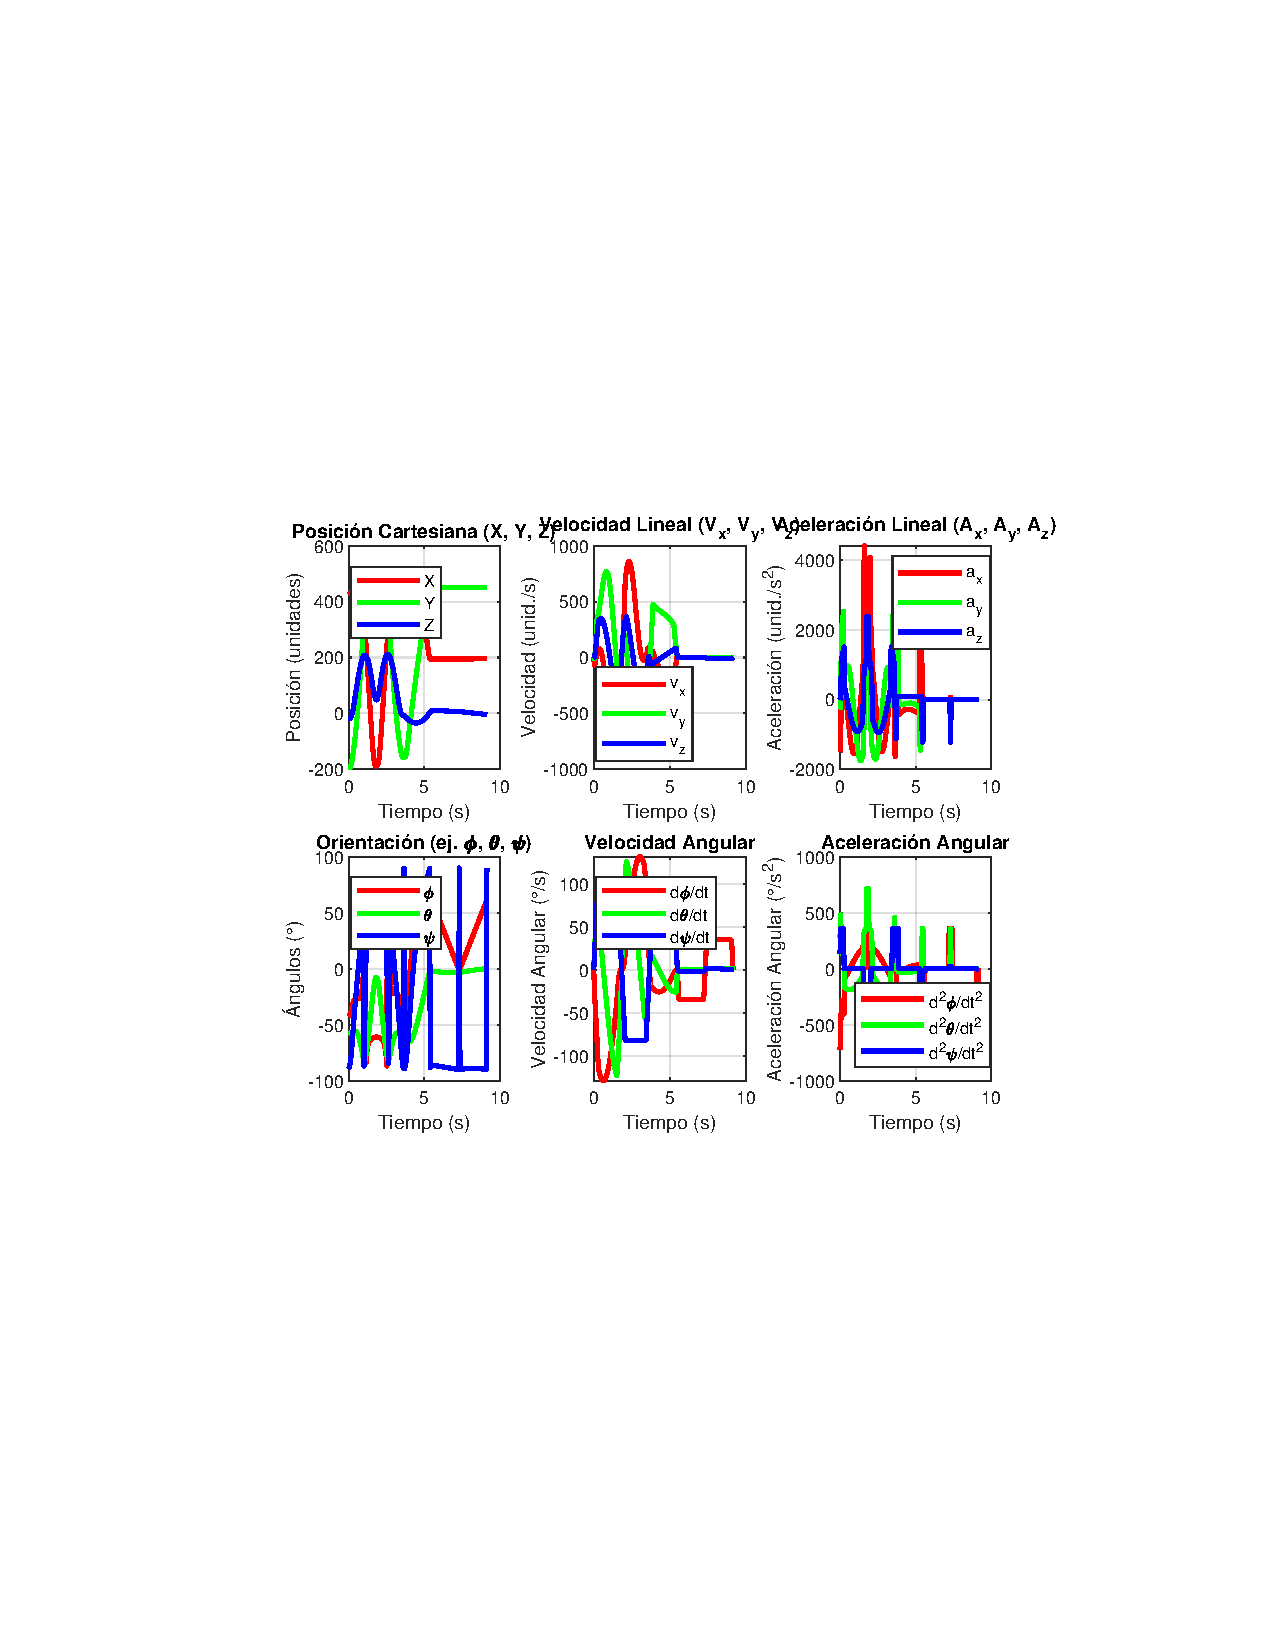
\includegraphics[width=\textwidth, trim={4cm 1cm 4cm 1cm}, clip]{Graficas_inversa_robot_final.pdf}
		\caption{Primera gráfica}
		\label{fig:inversa1}
	\end{subfigure}
	\hfill
	\begin{subfigure}[c]{0.495\textwidth}
		\centering
		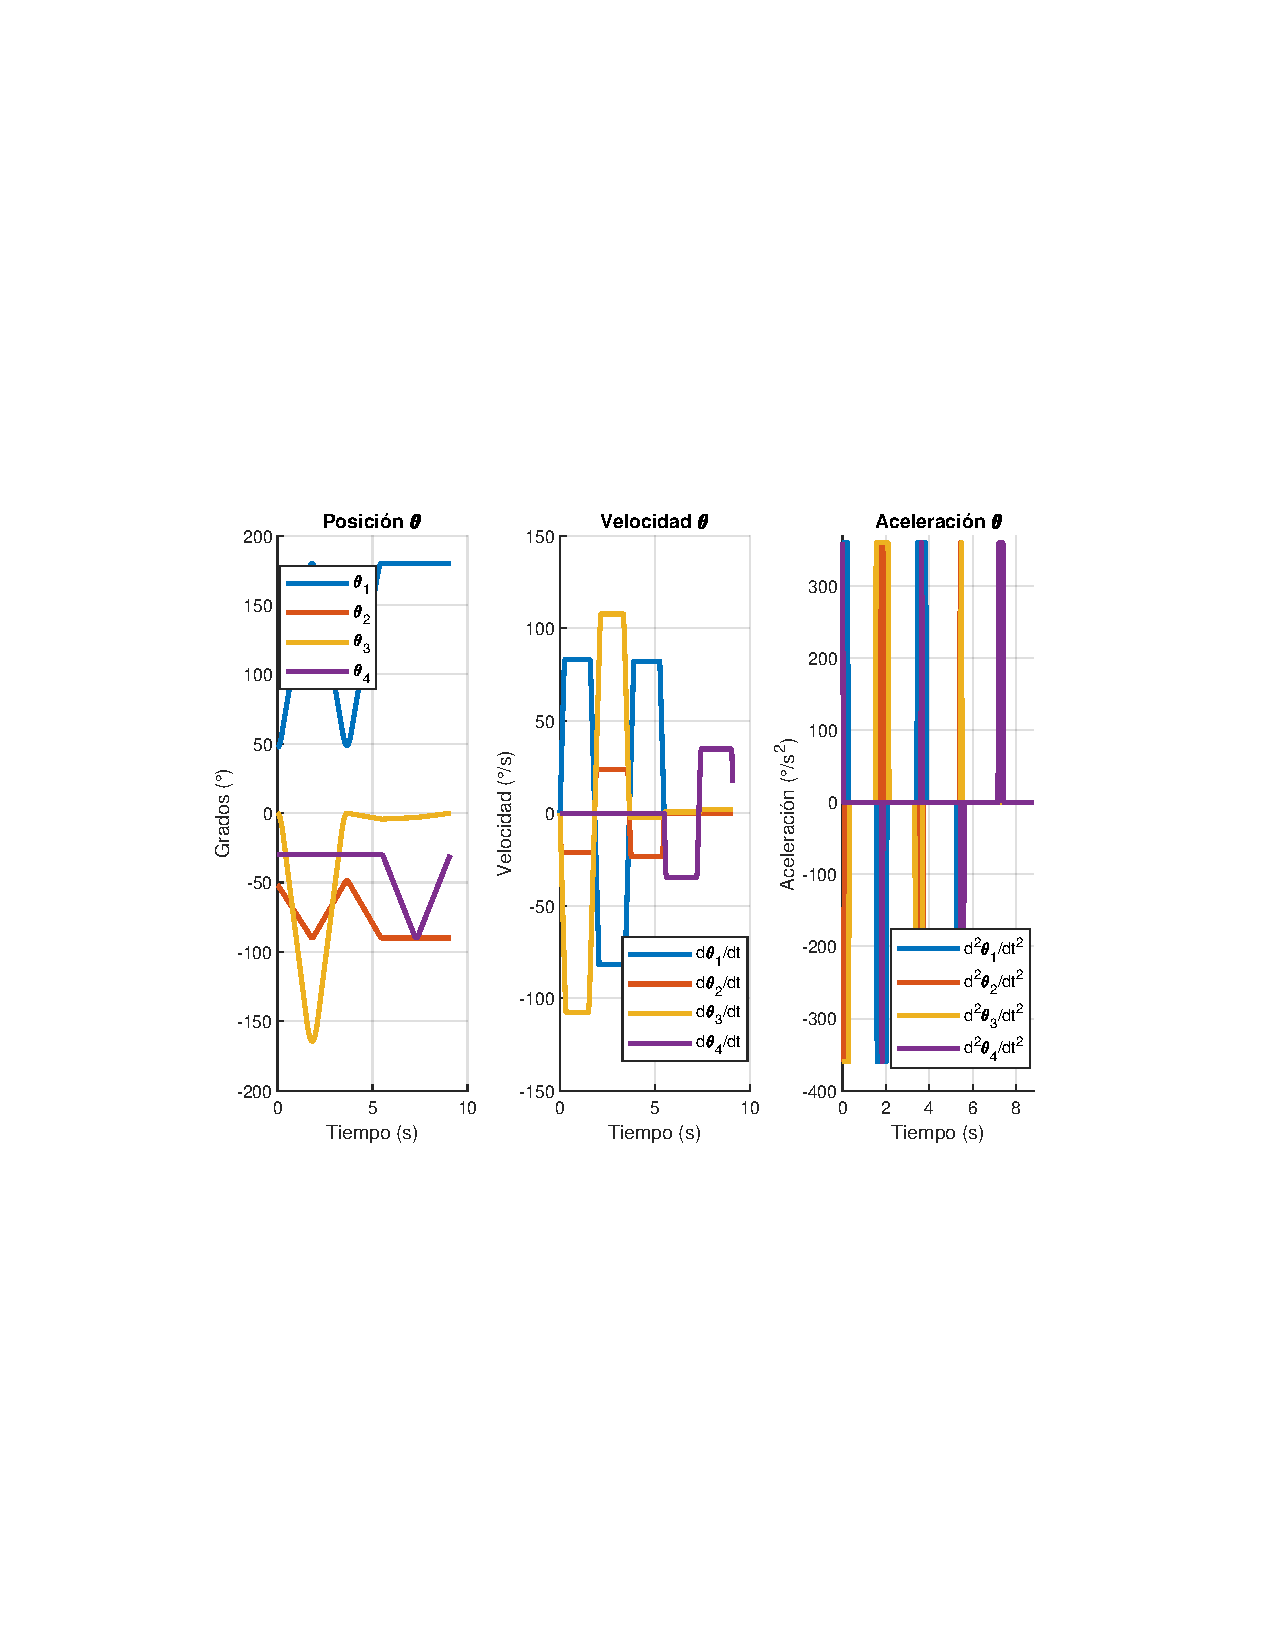
\includegraphics[width=\textwidth, trim={4cm 1cm 4cm 1cm}, clip]{Graficas_inversa2_robot_final.pdf}
		\caption{Segunda gráfica}
		\label{fig:inversa2}
	\end{subfigure}
	\captionsetup{aboveskip=2pt}
	\caption{Gráficas de cinemática inversa generadas en MATLAB.}
	\label{fig:cinematicaInversaFinal}
	\vspace{-3.5em}
	
\end{figure}
\vspace{5em} 

El siguiente conjunto de gráficas representa el comportamiento cinemático del robot obtenido mediante la \textbf{cinemática inversa}, resolviendo los ángulos articulares necesarios para que el efector final siga una trayectoria determinada en el espacio cartesiano. Estas gráficas permiten analizar cómo deben evolucionar las variables articulares para que el robot logre cumplir su trayectoria deseada.

\begin{itemize}
	\item \textbf{Posición Cartesiana (X, Y, Z)}\\
	Gráfica superior izquierda del conjunto (a).
	
	Muestra la trayectoria deseada del efector final expresada en coordenadas cartesianas. Se representa cómo varía la posición en los ejes $X$ (rojo), $Y$ (verde) y $Z$ (azul) a lo largo del tiempo.
	
	\textit{Interpretación:} el robot debe seguir una trayectoria definida que puede presentar comportamientos complejos u oscilatorios, lo cual implica una planificación precisa de movimientos articulares.
	
	\item \textbf{Velocidad Lineal ($V_x$, $V_y$, $V_z$)}\\
	Gráfica superior central.
	
	Representa la primera derivada temporal de la posición cartesiana. Indica la velocidad con la que se mueve el efector final en cada una de las direcciones espaciales.
	
	\textit{Interpretación:} las variaciones no uniformes y oscilatorias indican que el robot debe ajustar continuamente sus articulaciones para mantener la trayectoria deseada.
	
	\item \textbf{Aceleración Lineal ($a_x$, $a_y$, $a_z$)}\\
	Gráfica superior derecha.
	
	Muestra la segunda derivada de la posición, es decir, cómo cambia la velocidad lineal con el tiempo.
	
	\textit{Interpretación:} los picos abruptos de aceleración reflejan la necesidad de aplicar fuerzas articulares significativas en momentos clave de la trayectoria.
	
	\item \textbf{Orientación ($\phi$, $\theta$, $\psi$)}\\
	Gráfica inferior izquierda.
	
	Representa los ángulos de Euler: roll ($\phi$ - rojo), pitch ($\theta$ - verde) y yaw ($\psi$ - azul), que definen la orientación del efector.
	
	\textit{Interpretación:} los cambios en estos ángulos reflejan rotaciones necesarias del efector durante la trayectoria. Las oscilaciones pueden indicar ajustes finos para mantener una orientación deseada.
	
	\item \textbf{Velocidad Angular ($\dot{\phi}$, $\dot{\theta}$, $\dot{\psi}$)}\\
	Gráfica inferior central.
	
	Corresponde a la velocidad de cambio de los ángulos de orientación.
	
	\textit{Interpretación:} se observan zonas con alta velocidad angular, lo que sugiere reorientaciones rápidas del efector para ajustarse a la trayectoria deseada.
	
	\item \textbf{Aceleración Angular ($\ddot{\phi}$, $\ddot{\theta}$, $\ddot{\psi}$)}\\
	Gráfica inferior derecha.
	
	Representa la aceleración de los ángulos de orientación, es decir, cómo varía su velocidad angular.
	
	\textit{Interpretación:} los picos de aceleración angular reflejan momentos de cambio brusco en la orientación, indicando demandas importantes sobre los actuadores rotacionales.
	
\end{itemize}

\vspace{1em}

\noindent \textbf{Análisis de las variables articulares – Gráficas (b):}

\begin{itemize}
	\item \textbf{Posición articular $\theta$}\\
	Gráfica izquierda del grupo (b).
	
	Representa la evolución temporal de las posiciones angulares de las articulaciones del robot ($\theta_1$ a $\theta_6$).
	
	\textit{Interpretación:} se observa cómo cada articulación se ajusta en el tiempo para cumplir con la trayectoria cartesiana. Cambios suaves indican movimientos continuos, mientras que saltos o pendientes pronunciadas pueden señalar trayectorias exigentes o cercanas a singularidades.
	
	\item \textbf{Velocidad articular $\dot{\theta}$}\\
	Gráfica central del grupo (b).
	
	Muestra la velocidad angular de cada articulación.
	
	\textit{Interpretación:} velocidades elevadas pueden ser indicativas de reconfiguraciones rápidas necesarias para mantener la trayectoria deseada, lo cual requiere una capacidad de respuesta alta por parte de los motores.
	
	\item \textbf{Aceleración articular $\ddot{\theta}$}\\
	Gráfica derecha del grupo (b).
	
	Representa la aceleración angular en cada articulación.
	
	\textit{Interpretación:} valores altos de aceleración pueden indicar esfuerzos importantes sobre los actuadores, y podrían requerir suavizado de trayectoria para evitar sobrecarga mecánica o daños.
	
\end{itemize}

\vspace{1em}

\noindent \textbf{Figura 4.2:} Gráficas de cinemática inversa generadas en MATLAB. Comparan la trayectoria deseada con las exigencias articulares necesarias para cumplirla.


\subsubsection{Gazebo y RViz}
\begin{figure}[H] 
	\centering
	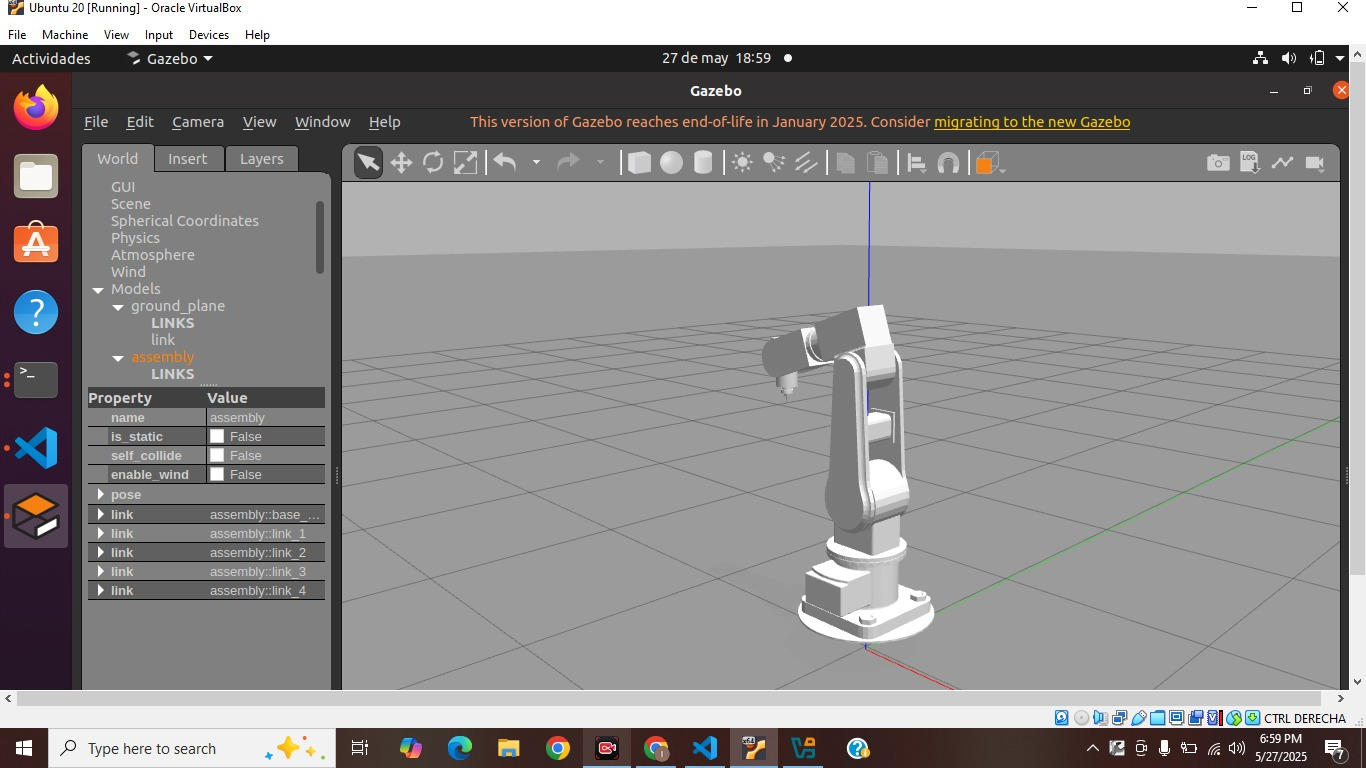
\includegraphics[width=0.8\textwidth]{RobGazebo.jpeg}
	\caption{Robot en Gazebo en posición inicial.}
	\label{fig:RobGazebo}
\end{figure}

\begin{figure}[H] 
	\centering
	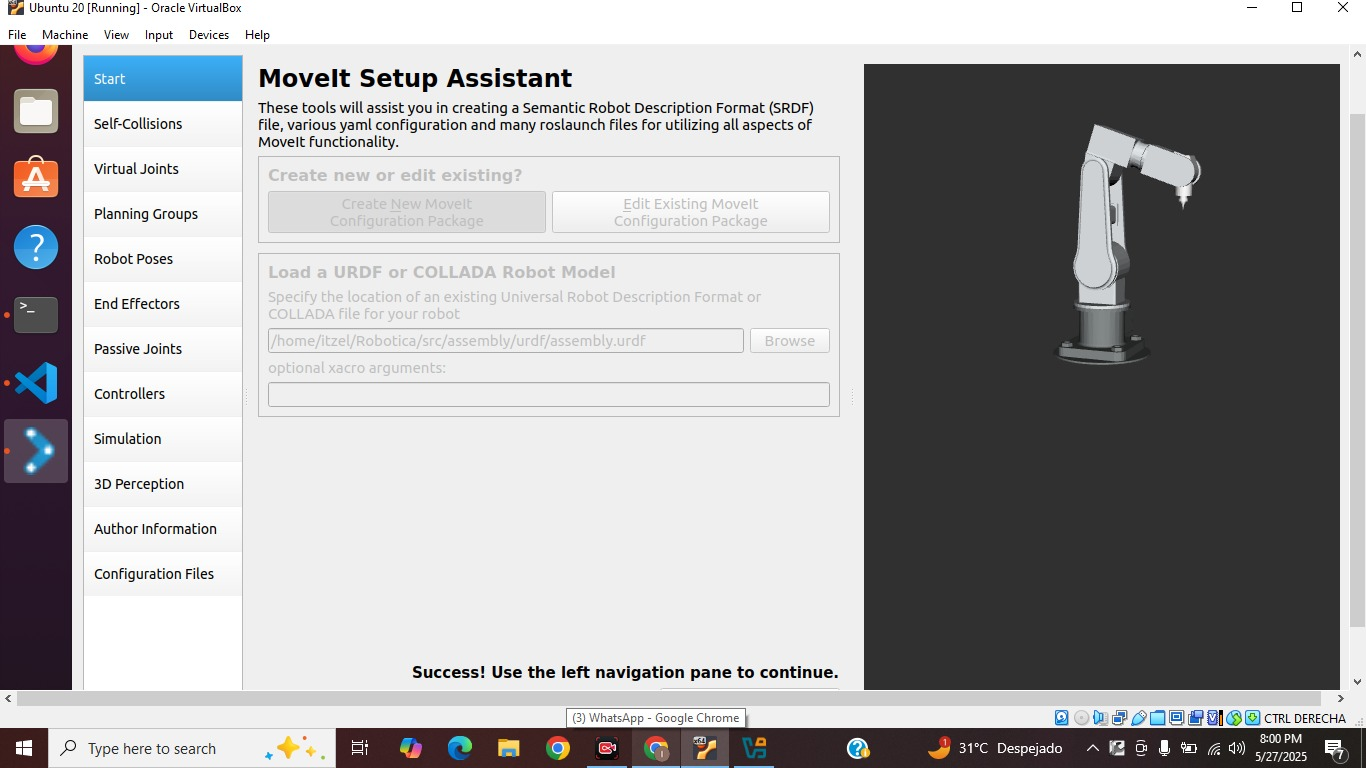
\includegraphics[width=0.8\textwidth]{moveit.jpeg}
	\caption{Move It Setup Assistant - Preview}
	\label{fig:moveit}
\end{figure}

\begin{figure}[H] 
	\centering
	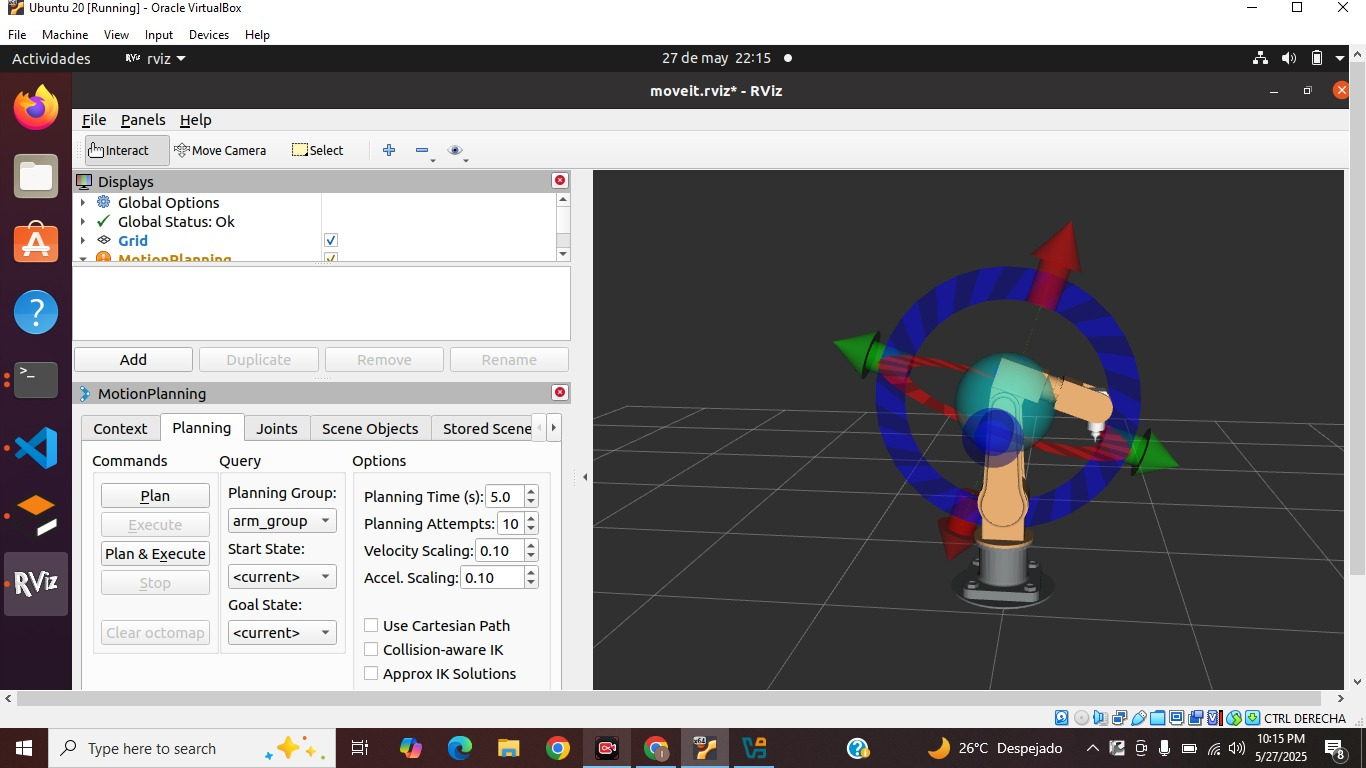
\includegraphics[width=0.8\textwidth]{Robenmoveit.jpeg}
	\caption{Robot en moveit.rviz* - RViz.}
	\label{fig:Robrviz}
\end{figure}
\paragraph{Análisis de Movimiento en Simulación.}

En las pruebas de simulación se observaron tres movimientos principales del robot \textit{Assembly}. El primero consiste en un movimiento descendente del brazo, simulando una acción de soldadura: el brazo baja de forma controlada y la punta del extremo se desplaza hacia arriba y hacia abajo, representando el recorrido dinámico de una soldadura.

En la segunda prueba, el robot se movió con su torque máximo, realizando un desplazamiento más rápido y firme, con el brazo orientándose hacia la derecha, simulando una acción potente, como si necesitara alcanzar o empujar en esa dirección.

Por otro lado, en la prueba con torque mínimo, el movimiento fue más lento y suave, y el brazo realizó un desplazamiento hacia arriba, mostrando un control más delicado, útil para tareas de precisión o posicionamiento cuidadoso.

Estos movimientos permitieron evaluar el desempeño del robot en diferentes condiciones de fuerza y velocidad.
